In this chapter we will do further analyses of the model results with particular
emphasis on the AttentionSegRank architecture due to it's better performance
and explainability. On section one we will discuss the effects of using semantic segmentation
on neural network  training. Section 2 will show the quantitative relationship between
segmentation, attention and the perception quantification. And finally, section 3 we will
analyze the implications of this method on model explainability.

\section{Effect of semantic segmentation on learning}
As was already mentioned on section \ref{sec:training}, adding a fixed segmentator to
the neural network architecture resulted in a reduction of performance along with a considerable
reduction of overfitting. The behavior was expected when fully replacing the CNN features,
due to the reduced expressiveness of the segmentation and the lack of finetuning, but
unexpectedly, although it is reduced, this behavior persists when combining the fixed
segmentation with the finetuned ResNet50 through the attention layer. We conclude from this
that restricting the attention weights to the shapes and classes given by the segmentation
has a regularizing effect on learning, reducing the model capacity even when the amount of trainable
weights is maintained.

In the case of the PlacePulse dataset this is not a problem since
all traditional deep models suffer of significant overfitting. It remains an interesting research
question  if these behaviors will transfer to other tasks and datasets.

\begin{figure}[ht]
	\begin{center}
	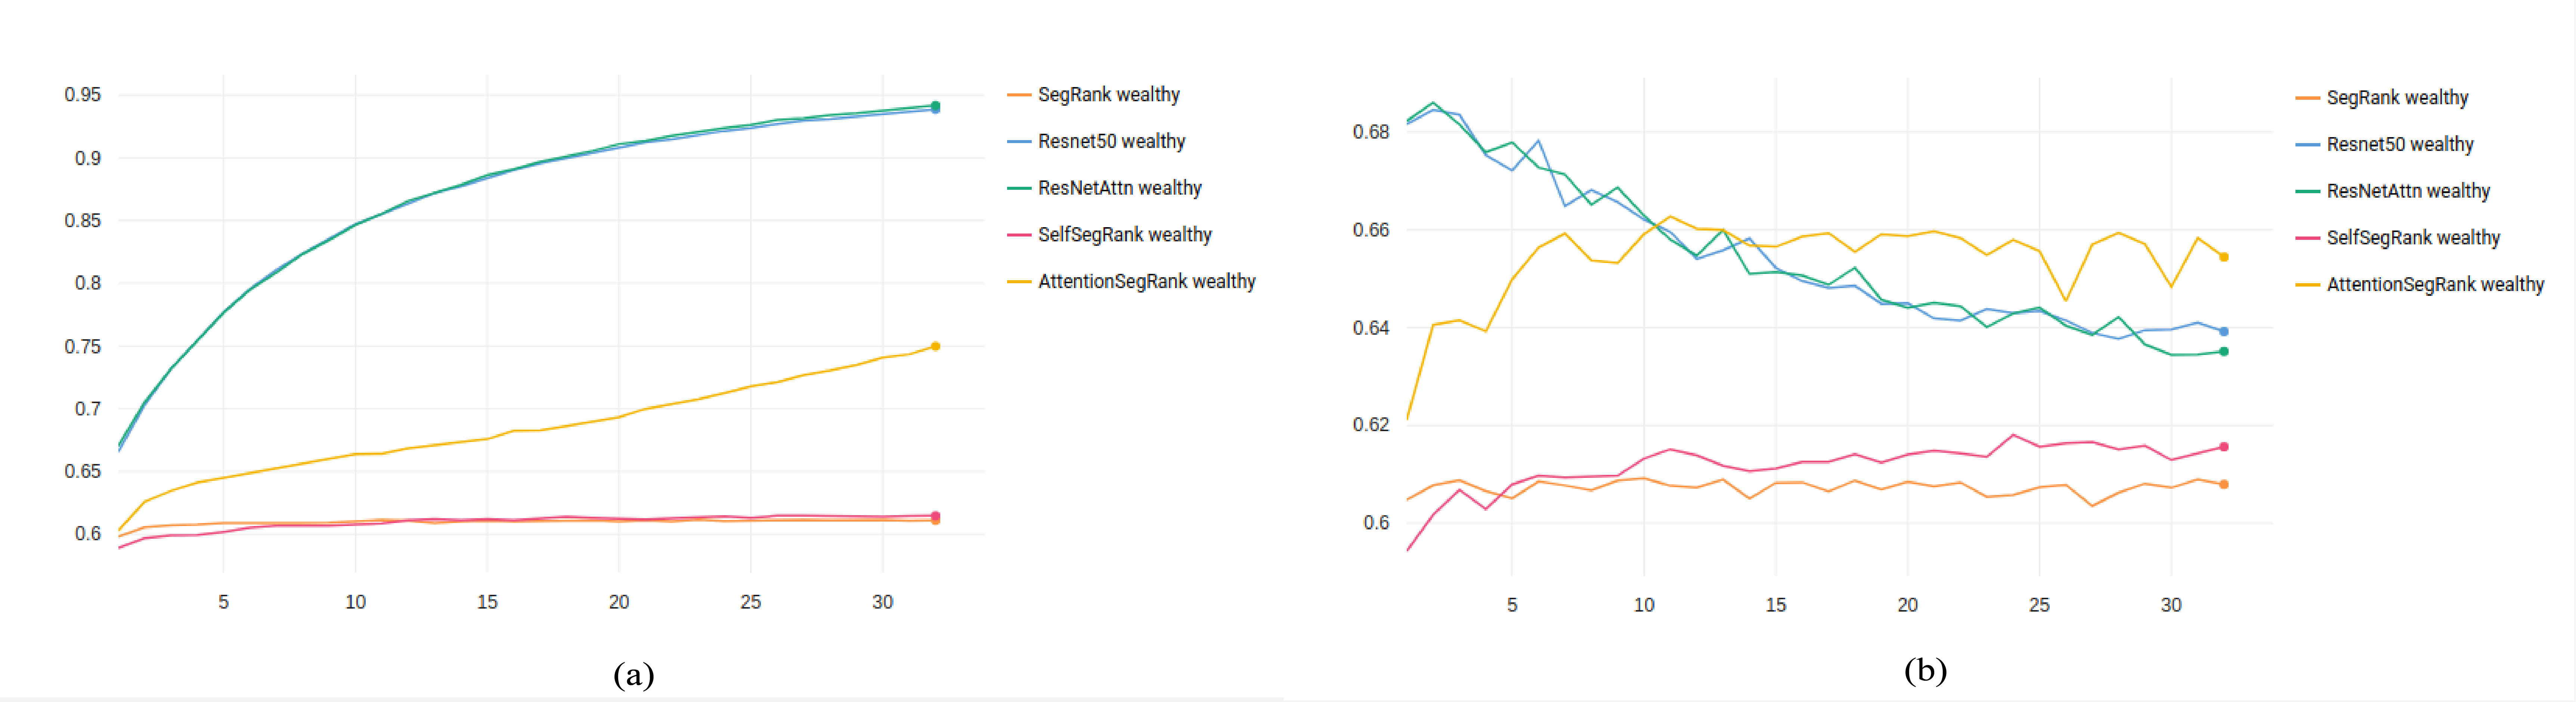
\includegraphics[width=1\textwidth]{./figures/wealthy_graph.png}
	\caption[Wealthy Training curves]{
        Wealthy accuracy vs epoch learning curves on training (a) and validation (b).
        }
	\label{fig:wealthy_graph}
	\end{center}
\end{figure}


\section{Relationship between urban perception and semantic segmentation}

\section{Relationship between urban perception and attention}

\section{Effect of attention over semantic segmentation on model explainability}